\chapter{基于乘法器库的近似逻辑综合}


广义的逻辑综合可分为传统逻辑综合、精确逻辑综合(Exact logic synthesis)和近似逻辑综合三类。
其中,传统逻辑综合(通常简称为逻辑综合)在整个芯片设计流程中处于最上游的位置,是指将数字电路的高抽象级描述(通常是指寄存器传输级),在功能一致的前提下经过布尔函数化简、优化后,转换到的逻辑门级别的网表的过程,其性能对芯片最终的面积和延迟起决定性作用。
精确逻辑综合(可简称为精确综合)要求在给定的约束下找到电路的最佳实现,比如基于给定的门的种类和数量上限对布尔网络进行映射\cite{LS:exact_syn},属于传统逻辑综合中的一个细分研究方向。
近似逻辑综合包括两个方向,一个方向侧重于近似算术单元的生成,也被叫做近似电路综合;另一个方向更靠近传统逻辑综合,即基于已有的近似库对大型设计进行优化和映射。本文着重于传统逻辑综合中大规模电路的序列探索,以及和近似乘法器库结合后针对DNN加速器的近似逻辑综合研究。

\section{基于MFFC自适应超图划分的端到端强化学习逻辑优化框架}

\subsection{研究背景}

\subsubsection{Yosys和ABC}

\begin{figure}[!htbp]
    \centering
    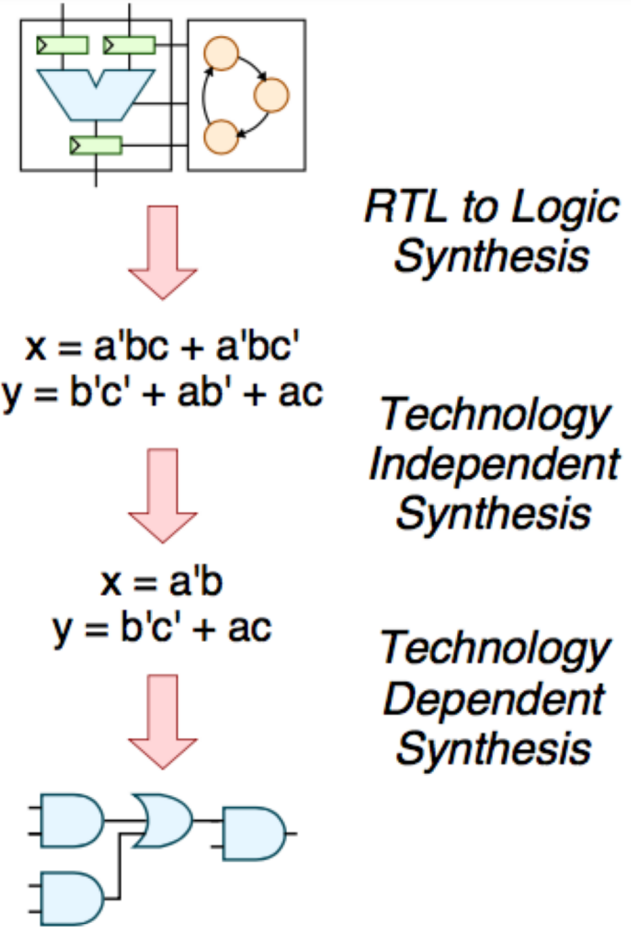
\includegraphics[width=0.4\linewidth]{./figs/LS-flow.png}
    \caption{传统逻辑综合流程图}
    \label{LS:flow}
\end{figure}

\begin{figure}[!htbp]
    \centering
    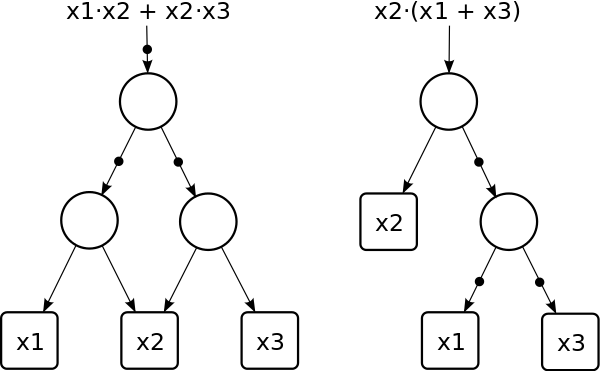
\includegraphics[width=0.6\linewidth]{./figs/LS-two_AIG.png}
    \caption{函数$x_2 (x_1 + x_3)$的两种不同的AIG实现}
    \label{LS:two_AIG}
\end{figure}


图\ref{LS:flow}展示了传统逻辑综合的流程图,首先将用户设计的寄存器传输级电路读入并解析,然后进行一系列工艺无关的逻辑优化操作,最后进行工艺相关的映射,生成门级网表。在现代EDA工具中,解析后电路中的组合逻辑部分通常由一个有向无环图进行表示,被称为布尔网络\cite{FPGA:CLB_Anderson},网络中的节点代表逻辑函数,边代表连接关系,逻辑综合进行的一系列优化及映射操作都基于该网络实现。
在一个布尔网络中\cite{LS:exact_rewriting,FPGA:Jason_Cong_1993,LS:Verification_after_synthesis},一个节点的扇入(Fanin)和扇出(Fanout)分别指该节点的输入节点和输出节点;
假设存在一条路径从节点$v$到节点$w$,则$v$是$w$的传递扇入(Transitive fanin),$w$是$v$的传递扇出(Transitive fanout);
网络的主要输入(Primary Inputs, PIs)是指所有的无扇入节点,网络的主要输出(Primary Outputs, POs)是指所有与外部相连的节点;
一条路径的长度指经过的节点数目;
节点的深度或级数指从网络的所有主要输入到该节点的所有路径中最长路径的长度;
最大节点深度被称为网络的深度。

% 图\ref{LS:boolean_net}展示了一个简单的布尔网络的示意图,可以看作是有5个输入、6个输出、7个节点、16条边的DAG,

% \begin{figure}[!htbp]
%     \centering
%     \includegraphics[width=0.8\linewidth]{./figs/LS-boolean_net.png}
%     \caption{一个简单的布尔网络示意图}
%     \label{LS:boolean_net}
% \end{figure}

AIG(And-Inverter Graph)是目前一种被广泛用来对逻辑函数进行表示和优化的有向无环图\cite{LS:AIG},在AIG中,节点分为主要输入节点、主要输出节点和2输入的与门节点三种类型,边包括取反和不取反两种情况,主要输入节点没有输入边,主要输出节点可能有输出边。一个逻辑函数可由不同结构的AIG表示,图\ref{LS:two_AIG}展示了函数$x_2 (x_1 + x_3)$两种不同的AIG实现。基于AIG,由Berkeley大学研发的的逻辑综合与验证工具ABC\cite{LS:ABC}在学术界和工业界获得了广泛的关注和赞誉。ABC可以对AIG进行逻辑优化和工艺映射,逻辑优化的目标是最小化AIG的规模和深度,映射目标是最小化LUT或ASIC电路的面积和延迟。


% 研究表明\cite{LS:structural_bias},AIG的映射结果会受到结构偏差(Structural bias)问题的影响,具体来说,同一个AIG进行不同的变换后会有不同的映射结果,且质量差别较大,这是由于AIG结构的不同导致映射器无法发现更优的解。图\ref{LS:structural_bias}展示了结构偏差问题的存在对LUT映射质量产生影响的一个示例,

% \begin{figure}[!htbp]
%     \centering
%     \includegraphics[width=\linewidth]{./figs/LS-structural_bias.png}
%     \caption{结构偏差问题影响LUT映射质量的一个示例}
%     \label{LS:structural_bias}
% \end{figure}


在逻辑优化阶段,ABC存在着许多不同的命令对AIG进行变换和化简,典型的命令包括balance, refactor, rewrite等,不同的优化命令会对AIG产生不同的优化效果,开发人员根据经验预先设定了一些优化脚本(如resyn2)对不同的电路进行使用。然而,不同命令的组合及顺序对逻辑优化的效果有很大影响,并且当优化进行到一定程度后,继续优化并不一定会对后续的映射操作起到正面效果\cite{LS:PIMap},因此必须针对不同的电路提供不同的优化序列,以达到对不同电路都能实现良好提升的目的。为给定的布尔逻辑网络寻找较优逻辑优化命令组合的问题被称为序列探索。

ABC能够利用AIG对布尔网络进行有效地表示和变换,但在电路解析方面能力不足。目前使用最广泛的硬件描述语言(Hardware description language)是Verilog-2005,被大多数EDA工具支持。Yosys\cite{LS:yosys}是一款开源的Verilog解析工具,支持绝大部分Verilog-2005语法,与ABC结合能够完成从Verilog到门级网表的全流程工作。

\subsubsection{用来表示布尔网络的不同DAG形式}

(1)XAIG

\begin{figure}[!htbp]
    \centering
    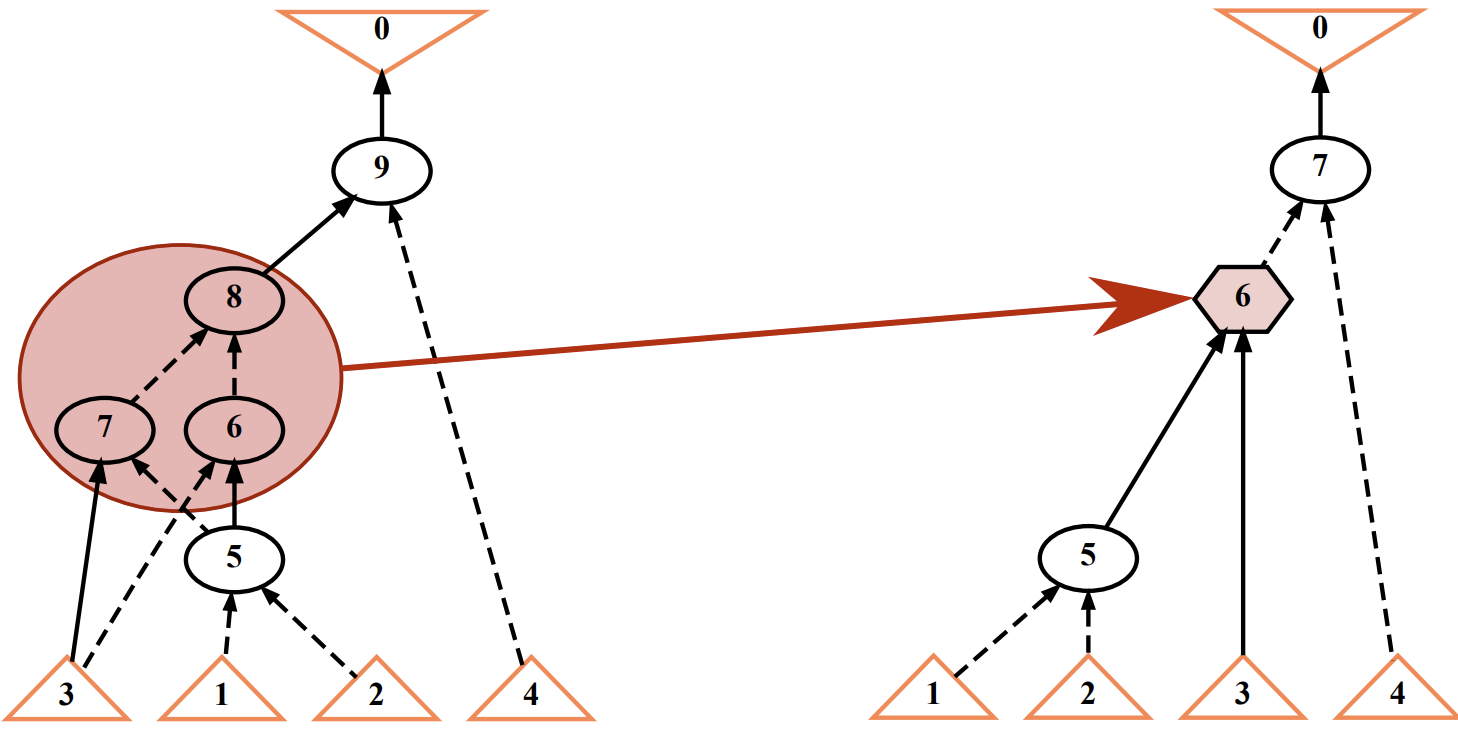
\includegraphics[width=0.75\linewidth]{./figs/LS-XAIG.png}
    \caption{函数$ \overline{ \overline{x_1 + x_2} \oplus x_3} \cdot \overline{x_4} $的AIG和XAIG,圆圈代表AND节点,六边形代表XOR节点,虚线边代表取反操作}
    \label{LS:XAIG}
\end{figure}

在AIG中,一个2输入异或门至少需要3个节点才能表示,这导致AIG无法对异或密集型电路进行高效地表示和优化,因此有工作提出了XAIG(Xor-And-Inverter Graph),在AIG中引入2输入的XOR节点,提高异或操作的表达效率\cite{LS:XAIG_Microelec_Relia,LS:XAIG_ddecs,LS:XAIG_iwls}。
图\ref{LS:XAIG}展示了函数$ \overline{ \overline{x_1 + x_2} \oplus x_3} \cdot \overline{x_4} $的AIG和XAIG,其中圆圈代表AND节点,六边形代表XOR节点,虚线边代表取反操作,可以看到XOR节点的引入能够降低图的规模。XAIG也被称为XAG(Xor-And Graph)。

(2)MIG

与XAIG的提出类似,有工作发现AIG能对控制电路进行高效地表达和变换,但对算术电路的操作效率较低,于是提出了适用于算术电路的MIG(Majority-Inverter Graph)\cite{LS:MIG}形式。在MIG中,除了输入节点外,每个节点表示一个3输入的Majority门,用符号$\langle \rangle$表示,定义为:
\begin{equation}
    \label{LS:MIG:Eq:Majority}
    \langle xyz \rangle = xy + xz + yz = (x + y) (x + z) (y + z)
\end{equation}

(3)XMG

对MIG引入3输入的XOR节点,能够提高某些函数的表达效率,对应的DAG实现被称为XMG(Xor-Majority Graph)\cite{LS:XMG_2017}。图\ref{LS:XMG}展示了函数$\langle x_1,x_2,(x_3 \oplus x_4) \rangle$分别在AIG、MIG和XMG中的表示,虚线代表取反操作,可以看到XMG使用的节点数目最少\cite{LS:XMG_2024}。

\begin{figure}[!htbp]
    \centering
    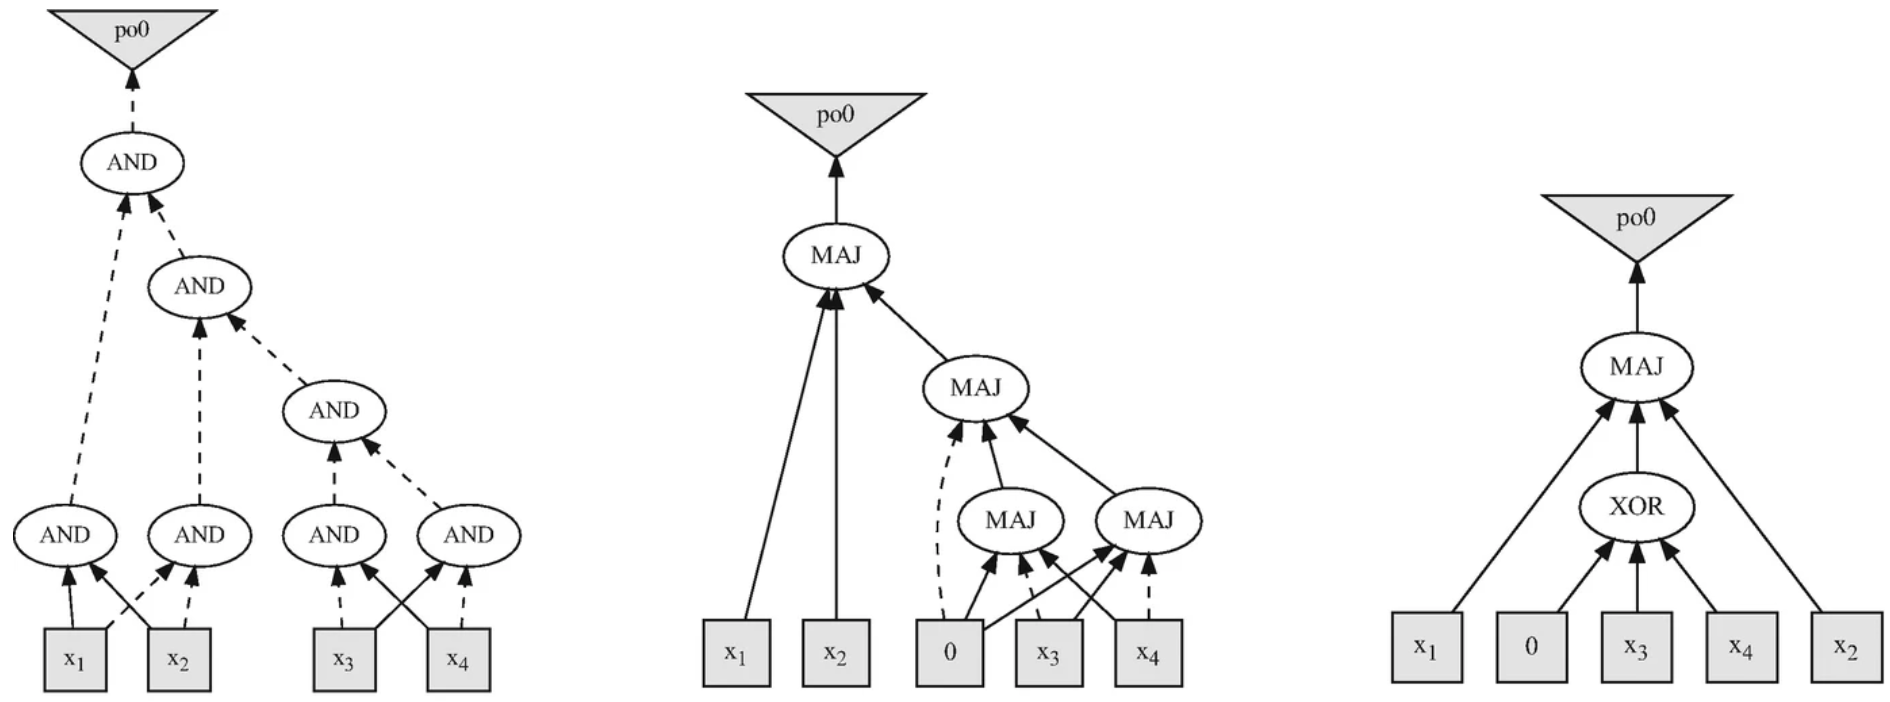
\includegraphics[width=\linewidth]{./figs/LS-XMG.png}
    \caption{函数$\langle x_1,x_2,(x_3 \oplus x_4) \rangle$分别在不同DAG中的表示,从左到右依次为:AIG、MIG、XMG,虚线代表取反操作}
    \label{LS:XMG}
\end{figure}

\subsubsection{MFFC} \label{MFFC}

在一个布尔网络中,节点$v$的一个锥(Cone)$C_v$是指$v$和$v$的传递扇入节点的集合(不包括网络的主要输入),锥中任意节点到$v$的路径都在锥内,$v$被称为锥的根节点,易知$v$可以有多个锥\cite{LS:exact_rewriting,FPGA:Jason_Cong_1993}。扇入节点数量小于等于$K$的锥被称为$K$可行锥($K$-feasible cone)\cite{FPGA:Jason_Cong_1999_cut_ranking}。

节点$v$在锥$C_v$下的一个割(Cut)是$C_v$的一个划分$(X,\overline{X})$,其中$\overline{X}$是$v$的一个锥。当$\overline{X}$是一个$K$可行锥时,割$(X,\overline{X})$被称为$K$可行割($K$-feasible cut)\cite{FPGA:Jason_Cong_1999_cut_ranking}。$\overline{X}$的扇入节点集合$L$满足以下两个性质:
\begin{itemize}
    \item 任意一条从网络的主要输入到节点$v$的路径至少会经过$L$中的一个元素;
    \item 对于$L$中的任何一个节点$l$,至少存在一条从主要输入到$v$的路径经过$l$且不经过$L$中的其他节点。
\end{itemize}
图\ref{LS:z_cone_two_cuts}展示了节点z的一个锥\{z,x,a,d,c,b,e\}和两个割\cite{FPGA:CLB_Anderson}cut1、cut2,易知cut1和cut2均是3可行割。
\begin{figure}[!htbp]
    \centering
    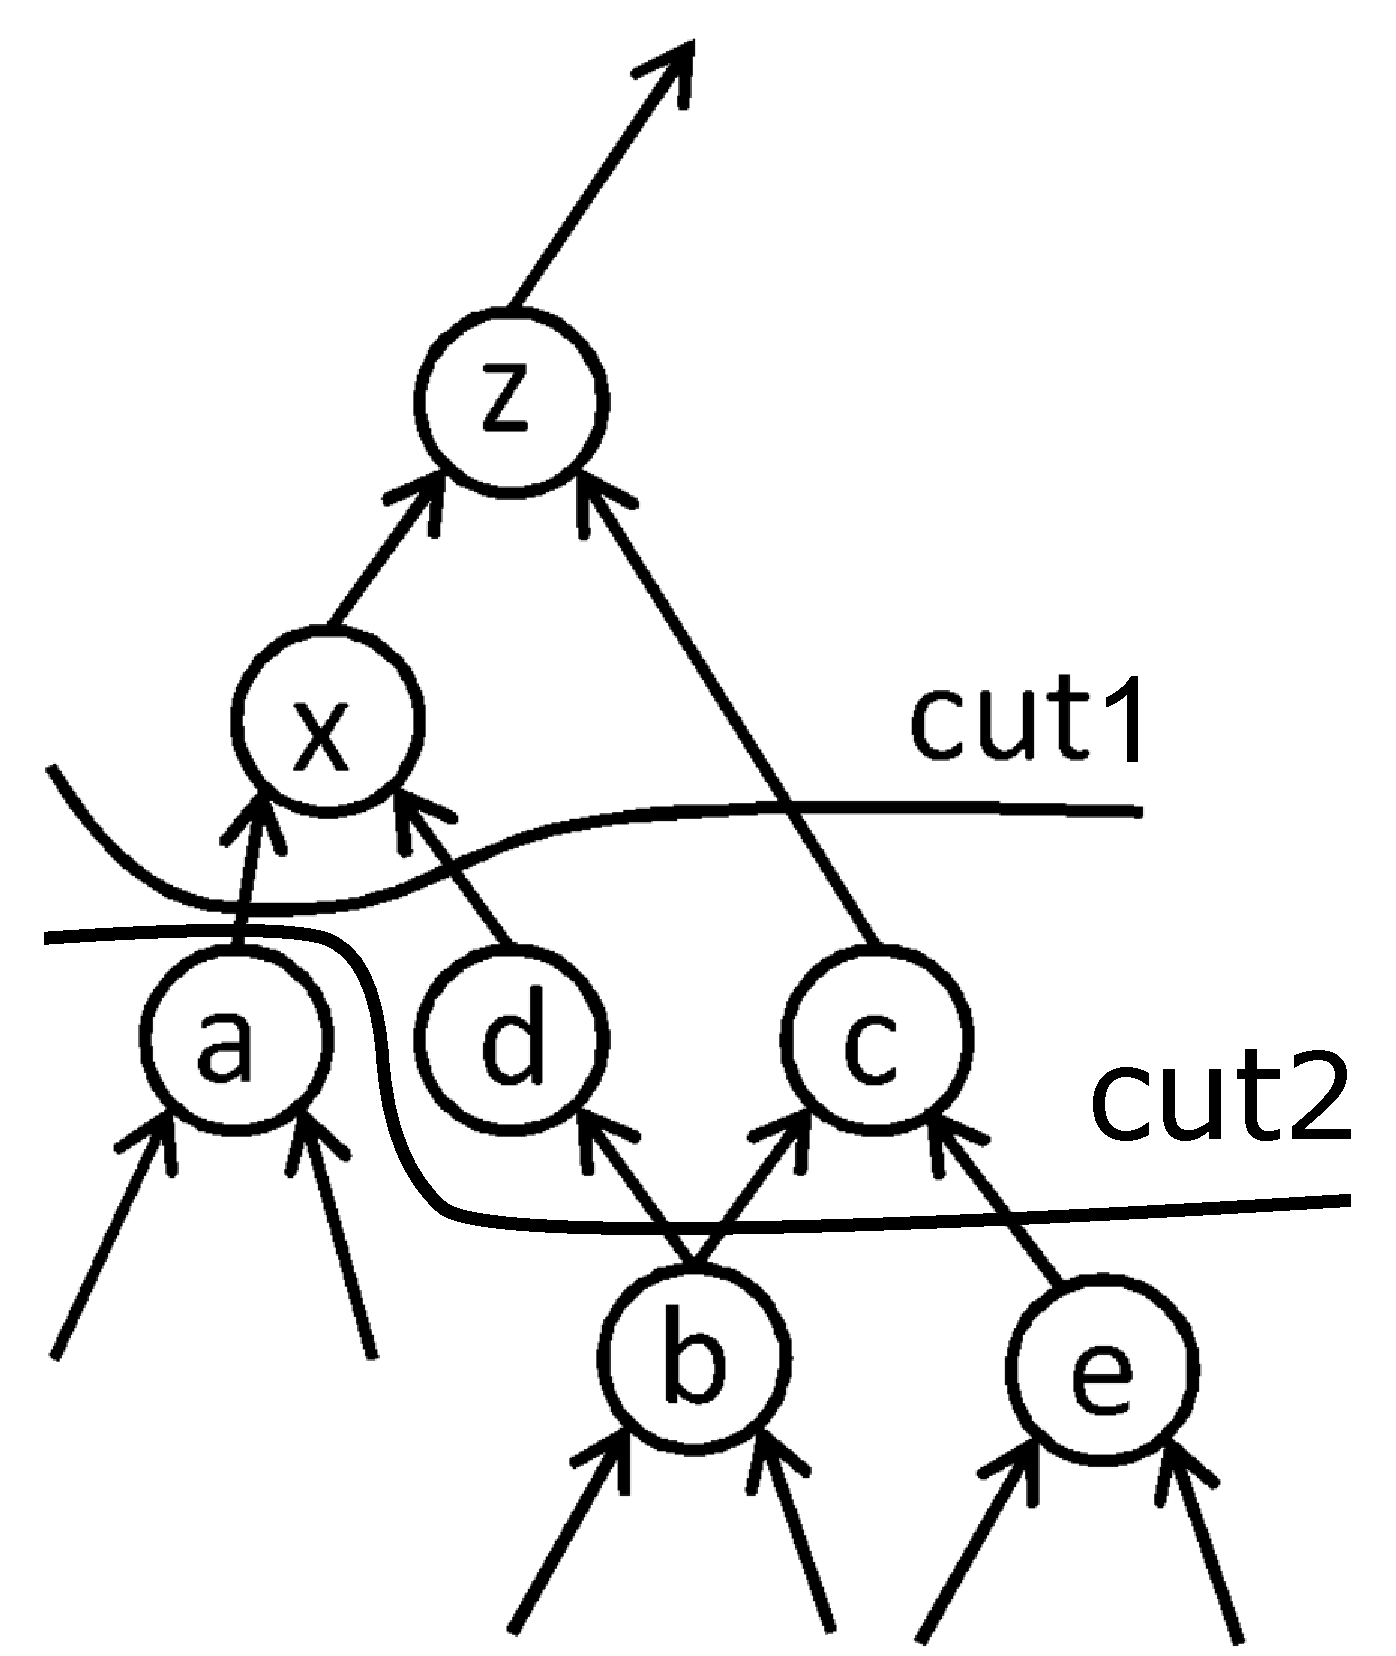
\includegraphics[width=0.4\linewidth]{./figs/LS-z_cone_two_cuts.pdf}
    \caption{节点z的一个锥\{z,x,a,d,c,b,e\}和两个割cut1与cut2}
    \label{LS:z_cone_two_cuts}
\end{figure}

若锥$C_v$内任意节点的扇出均在锥内,则称$C_v$为节点$v$的无扇出锥(Fanout Free Cone, FFC),$v$的所有无扇出锥中最大的那个被称为$v$的最大无扇出锥(Maximum Fanout Free Cone, MFFC),记为MFFC$_v$,易知MFFC有以下性质\cite{LS:exact_rewriting,FPGA:Jason_Cong_1993,FPGA:Jason_Cong_patition}:
\begin{itemize}
    \item 一个节点的MFFC有且只有一个;
    \item 若 $w \in \text{MFFC}_v$,则$\text{MFFC}_w \subseteq \text{MFFC}_v$;
    \item 两个MFFC要么不相交,要么一个包含另一个;
    \item $\text{MFFC}_v$中节点的值只会影响到$v$和$v$的传递扇出。
\end{itemize}
\begin{figure}[!htbp]
    \centering
    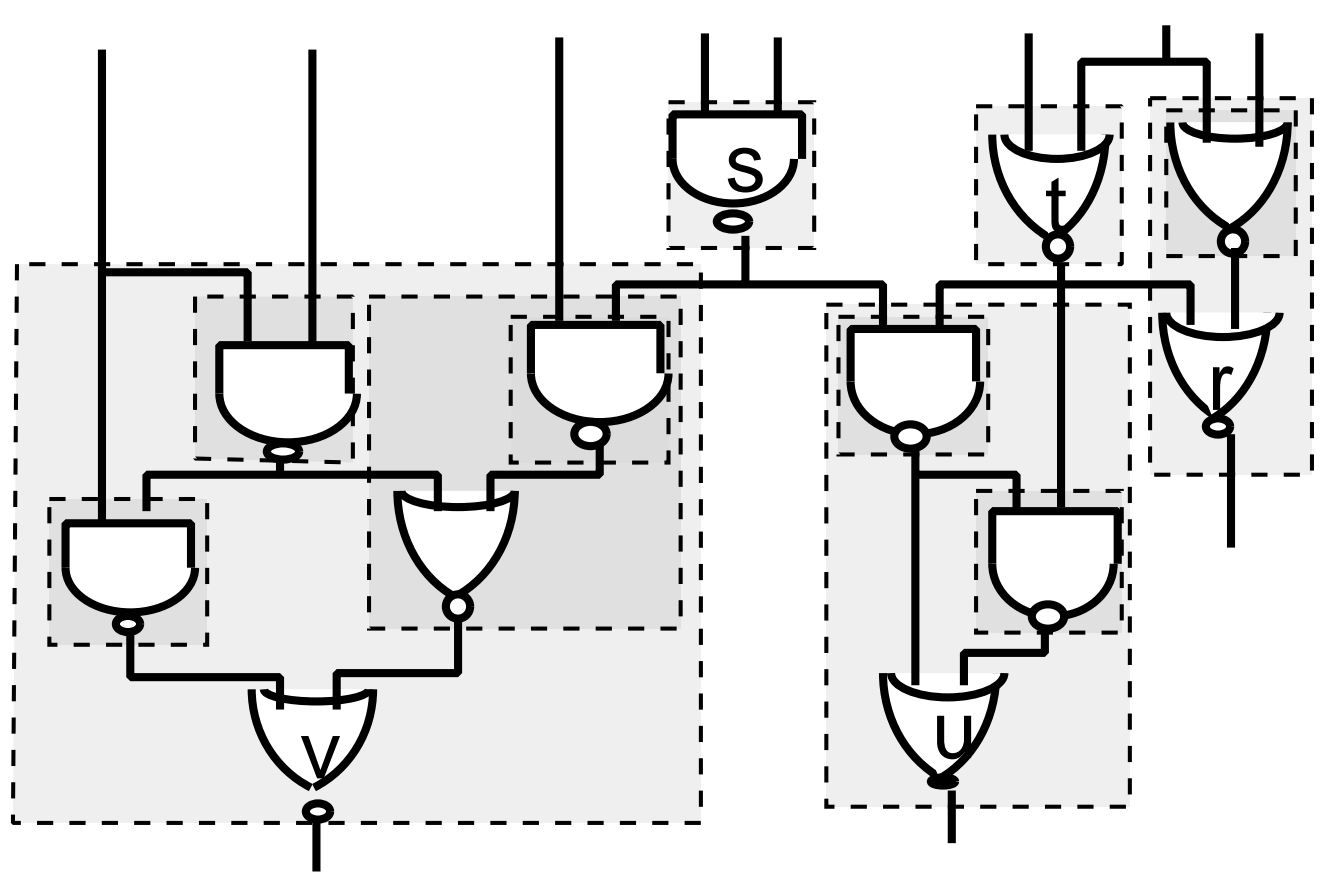
\includegraphics[width=0.6\linewidth]{./figs/LS-MFFC.png}
    \caption{不同节点的最大无扇出锥}
    \label{LS:MFFC}
\end{figure}
图\ref{LS:MFFC}展示了一个布尔网络中不同节点的MFFC,以不同灰度的阴影区域表示,可以看到各MFFC满足上述性质。


\subsubsection{电路划分}

当布尔网络的规模太大时,单个优化命令的运行时间变长,序列探索时单次迭代花费的时间显著增加,导致无法在一个可接受的时间范围内得到一个较优的命令组合,通过划分将大型网络分割成较小的子网络来并行地探索,能够大大减少运行时间。

(1)超图划分

一个网络的DAG图既可以转换成普通图(一条边只连接两个顶点),也可以转换成超图(一条边可以连接超过两个顶点),考虑到电路中的输出往往都是多扇出的,超图能够更好地体现其连接性,因此将电路转换成超图进行划分是一个较好的选择\cite{LS:LSOracle}。

\begin{figure}[!htbp]
    \centering
    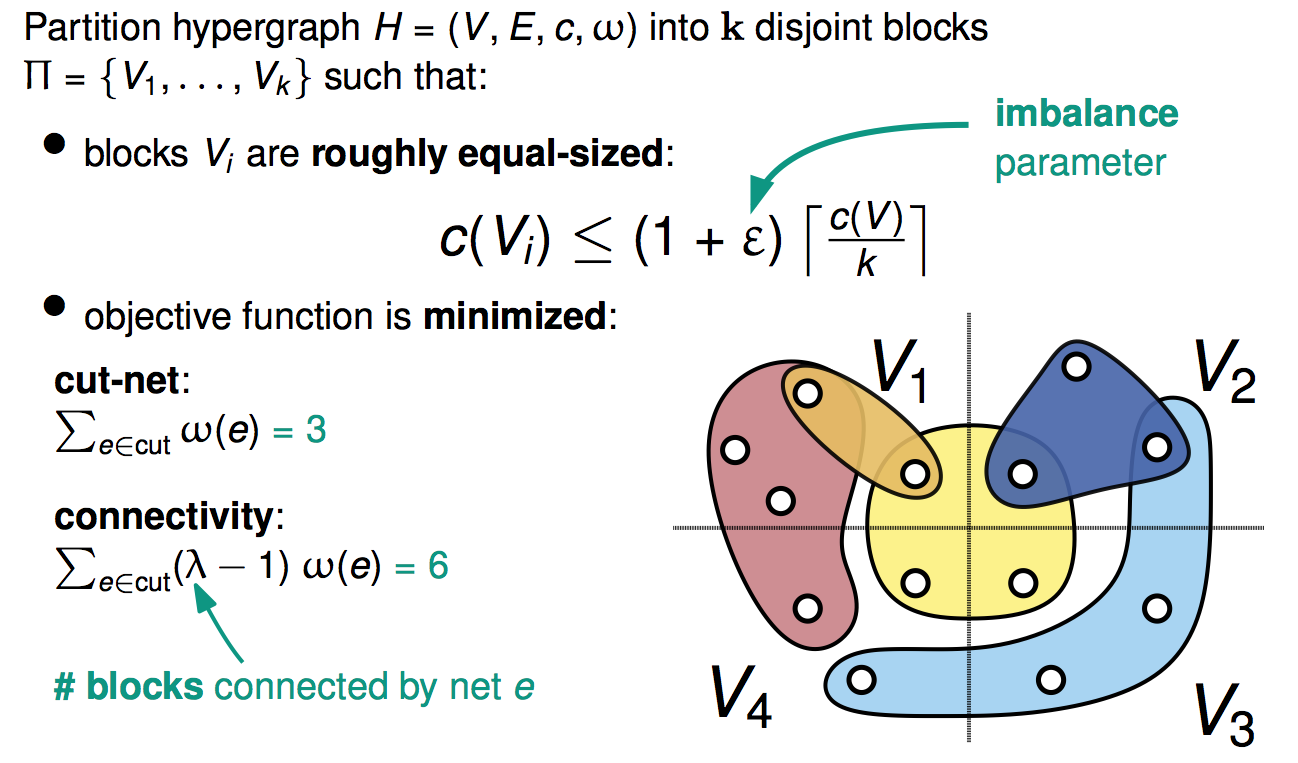
\includegraphics[width=0.8\linewidth]{./figs/Hypergraph_partition.png}
    \caption{超图划分问题的定义}
    \label{Hypergraph_partition}
\end{figure}

超图划分(Hypergrap partitioning)\cite{KaHyPar}能够对节点进行分类,将所有的节点划分为$k$个大致相等的部分,同时最小化基于边定义的目标函数,常见的目标函数有割边重要性和子图连通性,其中割边重要性是指被切割的超边的权重之和,而子图连通性则会同时考虑割边权重和割边连接的子图的数量。图\ref{Hypergraph_partition}展示了超图划分问题的定义以及两种目标函数的形式。
目前最常用的超图划分算法是多层(Multilevel)方法,由三个步骤组成:(1)粗化:对超图中不同连接紧密程度的点进行逐级合并以降低超图的规模;(2)初始划分:粗化完成后得到一个小的超图并对其进行初始划分;(3)细化:逐级分解原先合并的点并执行划分操作,每一次划分后利用局部搜索的方法来调整位于边界上的点以最小化目标函数,直到划分后子图的数目满足要求。

(2)自然划分

通常来讲,EDA工具对电路进行解析后生成布尔网络时会把寄存器与组合逻辑分开,将寄存器的输入变成组合逻辑的输出,将寄存器的输出变成组合逻辑的输入。有工作发现,良好设计的电路中流水线(Pipeline)技术充分,能够将整个电路“自然”地切分成数个均匀的组合逻辑块,转换成布尔网络后对应多个相互独立的DAG。基于此发现,文献\cite{Moucheng_Yang}提出了一种“自然划分(Natural partitioning)”的布尔网络分割方法,该方法基于ABC\cite{LS:ABC}实现,能够对一个大型AIG进行分簇,簇与簇之间没有连接,然后对所有的AIG簇并行地进行LUT映射以提高速度,对13个大型电路的测试结果表明,映射速度平均提高了5.76倍,面积略微增加了0.57\%,延迟保持不变。

(3)基于MFFC和带约束超图划分的有向无环划分

普通的超图划分并没有考虑DAG有向无环的特点,文献\cite{FPGA:Jason_Cong_patition}首先对一个网络进行遍历,利用MFFC缩小超图的规模,之后基于带约束的多层划分方法,提出了一个面向FPGA领域的有向无环划分方案,与普通超图划分相比割边数量更少、分割质量更高。

\subsubsection{强化学习}

强化学习是机器学习中的一个领域,强调一个智能体(Agent)如何基于环境(Environment)行动,以取得最大化的预期利益,是除了监督学习和非监督学习之外的第三种基本的机器学习方法。强化学习通过感知所处环境的状态(State)对动作(Action)的 反应(Reward),来指导更好的动作,从而获取最大的收益(Return)。以游戏为例,如果在游戏中采取某种策略可以取得较高的得分,那么就进一步“强化”这种策略,以期继续取得较好的结果。目前,强化学习在某些领域已经被证明了达到人类水平,甚至优于人类,比如早在2016年由谷歌研发的电脑围棋软件AlphaGo\cite{AI:AlphaGo}就已经击败了韩国围棋冠军李世石。

强化学习基于马尔科夫决策过程(Markov decision process),即当前状态包含了对未来预测所需要的所有信息,过去信息对未来预测不重要,关注点在于“探索未知领域”和“利用已有知识”的平衡,其实现算法分为有模型学习(Model-Based)和免模型学习(Model-Free)两类,其中免模型学习更容易实现,迁移性也更好,得到了广泛的研究。

\subsection{国内外研究现状}

\subsubsection{序列探索}

学术界提出了多种方法用来对逻辑综合中不同命令的组合及顺序进行探索,包括基于强化学习的方法、利用贝叶斯优化进行搜索、以及基于图神经网络进行预测等,下面分别进行介绍。

(1)基于强化学习的方法

\begin{figure}[!htbp]
    \centering
    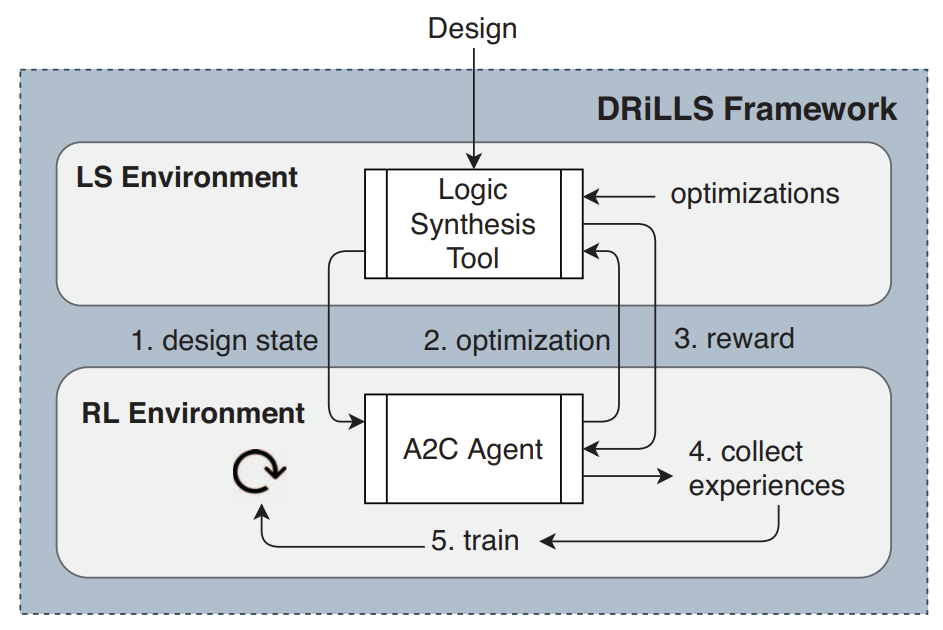
\includegraphics[width=0.7\linewidth]{./figs/LS-DRiLLS-framework.png}
    \caption{基于强化学习的序列优化方法DRiLLS的架构图}
    \label{LS:DRiLLS:Fig:framework}
\end{figure}

假设$\mathbb{A} = \{ a_1,\ a_2,\ a_3,\ \cdots,\ a_n \}$代表$n$个相互之间没有依赖的优化命令集合,$k$表示优化序列长度,则可能的命令组合情况一共有$n^k$种。
文献\cite{LS:DRiLLS}提出了一种基于强化学习的序列优化方法DRiLLS,DRiLLS利用A2C(Advantage Actor Critic)代理来探索序列空间。图\ref{LS:DRiLLS:Fig:framework}给出了DRiLLS的架构图,其中逻辑综合环境由Yosys和ABC实现,强化学习环境由A2C代理,与综合环境进行交互学习。DRiLLS将强化学习中的状态$state$定义为ABC中AIG的信息,包括主要输入输出数量、节点数、级数、寄存器数量、AIG中边的条数、以及AIG中反向边的数量。
同时,DRiLLS中强化学习的奖励函数是一个同时考虑面积和延迟的多目标函数,对于满足延迟约束且面积减少的优化序列,奖励最高(用+++表示),对于不满足延迟约束且面积增加的优化序列,奖励最低(用- - -表示),具体的奖励标准如表\ref{LS:DRiLLS:Table:reward}所示。

\begin{table*}[!htbp]
    \caption{DRiLLS中不同优化效果的序列对应的奖励情况}
    \centering
    \label{LS:DRiLLS:Table:reward}
    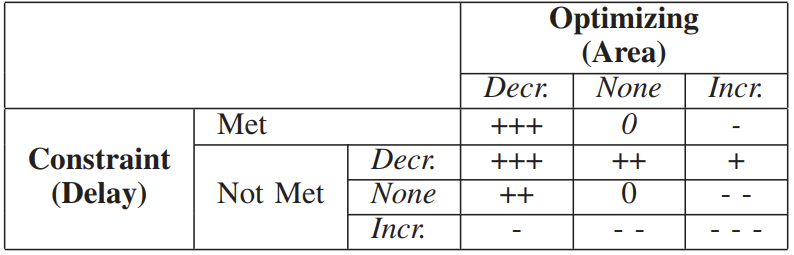
\includegraphics[width=0.7\linewidth]{./figs/LS-DRiLLS-reward_table.png}
\end{table*}

\begin{table*}[!htbp]
    \caption{实验结果}
    \centering
    \label{LS:DRiLLS:Table:results}
    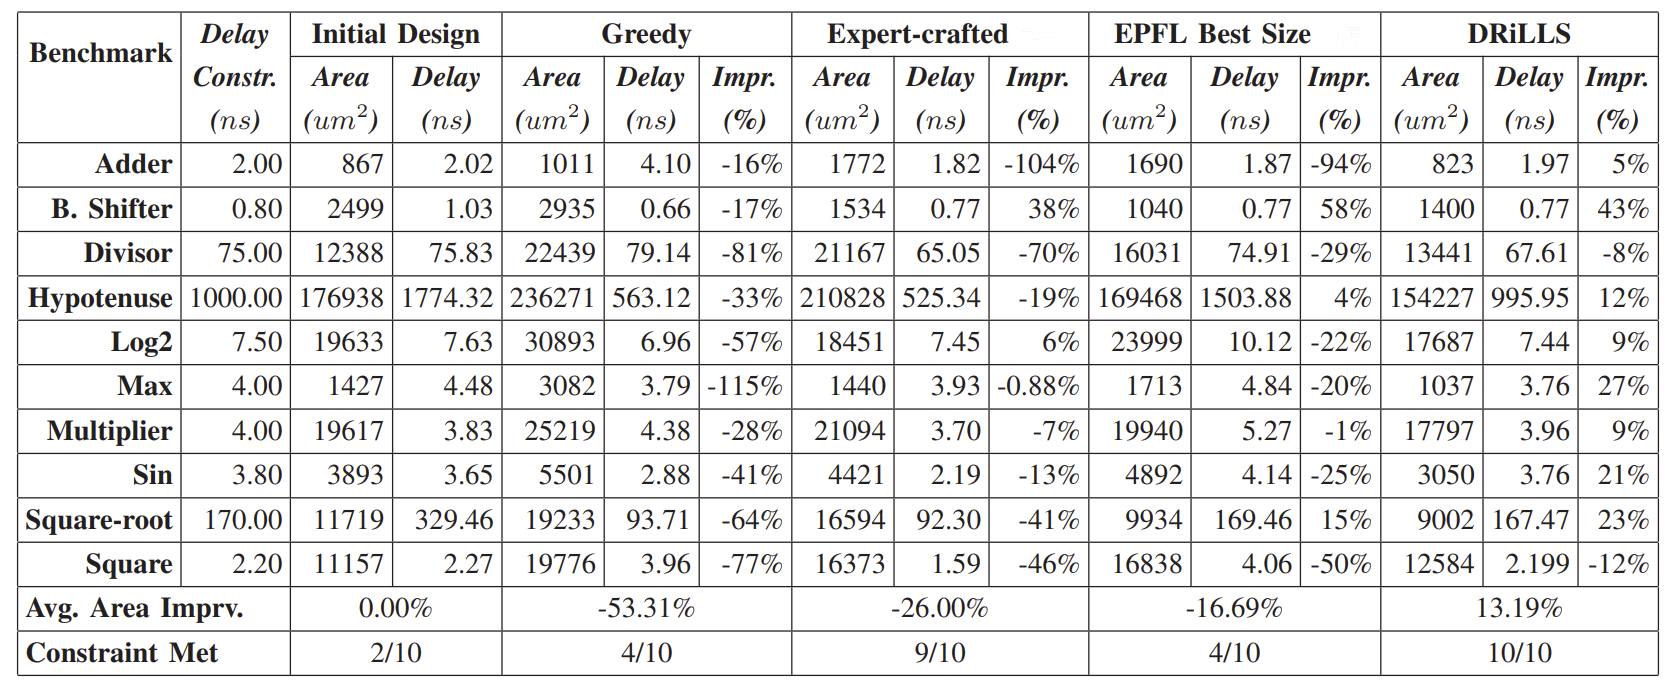
\includegraphics[width=\linewidth]{./figs/LS-DRiLLS-results.png}
\end{table*}

表\ref{LS:DRiLLS:Table:results}展示了基于ABC\cite{LS:ABC}和EPFL测试集\cite{LS:EPFL_benchs_iwls,LS:EPFL_benchs_github}通过4种方法包括贪婪算法(Greedy algorithm)、手工设计的优化序列\cite{LS:DRiLLS:hand_craft}(Expert-crafted)、已有的最佳记录、DRiLLS在开源的7nm工艺库\cite{ASAP7_github}上得到的实验结果,其中DRiLLS的延迟约束是初始的未优化的电路直接映射得到的延迟。
可以看到,DRiLLS在不同的电路上均满足了延迟约束,面积平均提高了13.19\%,这显示了DRiLLS多目标奖励函数的有效性。


(2)利用贝叶斯优化搜索

逻辑优化中的序列探索问题可以归结为黑盒优化问题,文献\cite{LS:BOiLS}提出了BOiLS,利用贝叶斯优化对命令的组合及顺序进行探索。基于ABC,对于一个给定的AIG,BOiLS的目标是在$n$个优化命令中找到一个长度为$K$的序列对电路进行优化,序列的好坏通过ABC进行LUT映射后来评估,其质量由下面的公式进行表达:
\begin{equation}
    \label{LS:BOiLS:Eq:QoR}
    QoR = \frac{Area(seq)}{Area(ref)} + \frac{Delay(seq)}{Delay(ref)}
\end{equation}
其中$Area(ref)$和$Delay(ref)$分别代表对原始电路用resyn2进行优化和映射后LUT的个数和级数,$Area(seq)$和$Delay(seq)$分别代表BOiLS找到的优化序列对原始电路进行优化和映射后LUT的个数和级数。在BOiLS中,考虑的优化命令包括:rewrite, rewrite -z, refactor, refactor -z, resub, resub -z, balance, fraig, sopb, blut, dsdb,序列大小$K=20$。

\begin{figure}[!htbp]
    \centering
    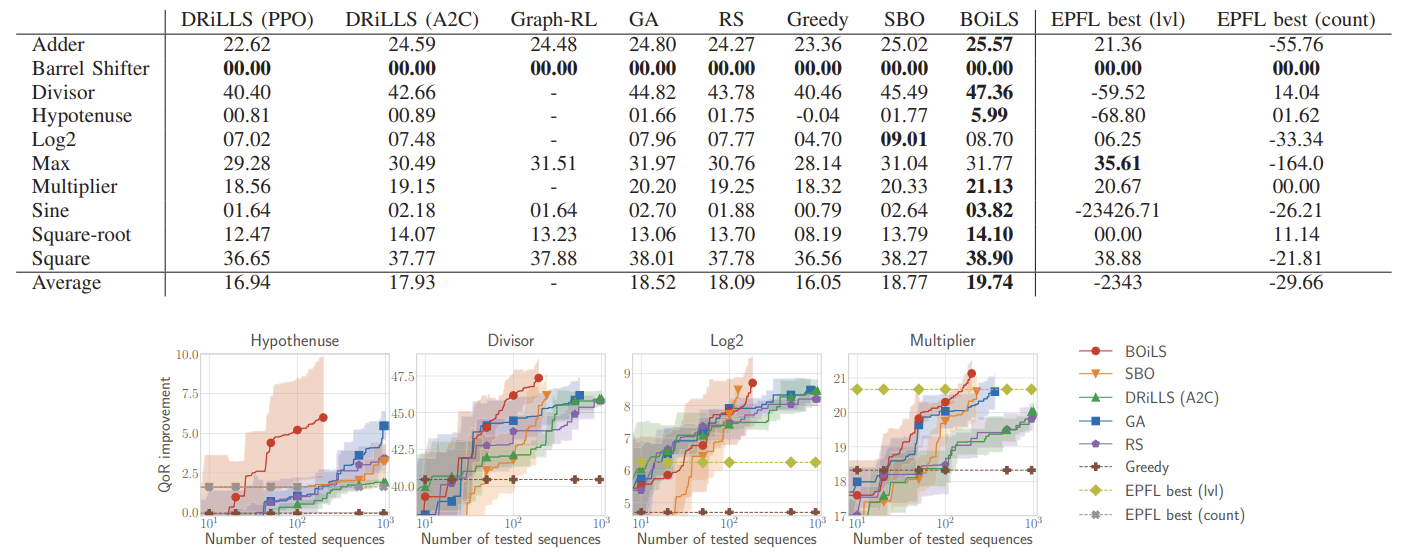
\includegraphics[width=\linewidth]{./figs/LS-BOiLS-results.png}
    \caption{不同序列探索方法在迭代200次后的LUT映射结果}
    \label{LS:BOiLS:Fig:results}
\end{figure}

基于EPFL电路集\cite{LS:EPFL_benchs_iwls,LS:EPFL_benchs_github},BOiLS与6个前沿工作进行了对比,包括:基于强化学习方法的DRiLLS\cite{LS:DRiLLS},标准贝叶斯优化(Standard Bayesian Optimization, SBO),遗传算法(Genetic Algorithm, GA),随机搜索(Random Search, RS),以及已有的最佳记录。每种方法限制的迭代次数为200,图\ref{LS:BOiLS:Fig:results}展示了不同方法的实验结果。可以看到,BOiLS在8/10个电路中都取得了最优结果,SBO在log2电路中效果最好,BOiLS紧随其后,显示了贝叶斯优化在逻辑综合序列探索中的巨大潜力。另外有趣的一点是,结果显示,基于强化学习的序列搜索方法DRiLLS看起来似乎并没有比随机搜索强多少。

(3)基于图神经网络的方法

图卷积网络(Graph Convolutional Network, GCN)是一种用于处理图数据的深度学习模型,其目标是将传统的卷积神经网络和递归神经网络等深度学习方法扩展到图结构数据如社交网络、推荐系统、生物信息学等领域,填补深度学习对图数据处理方式的空缺。

\begin{figure}[!htbp]
    \centering
    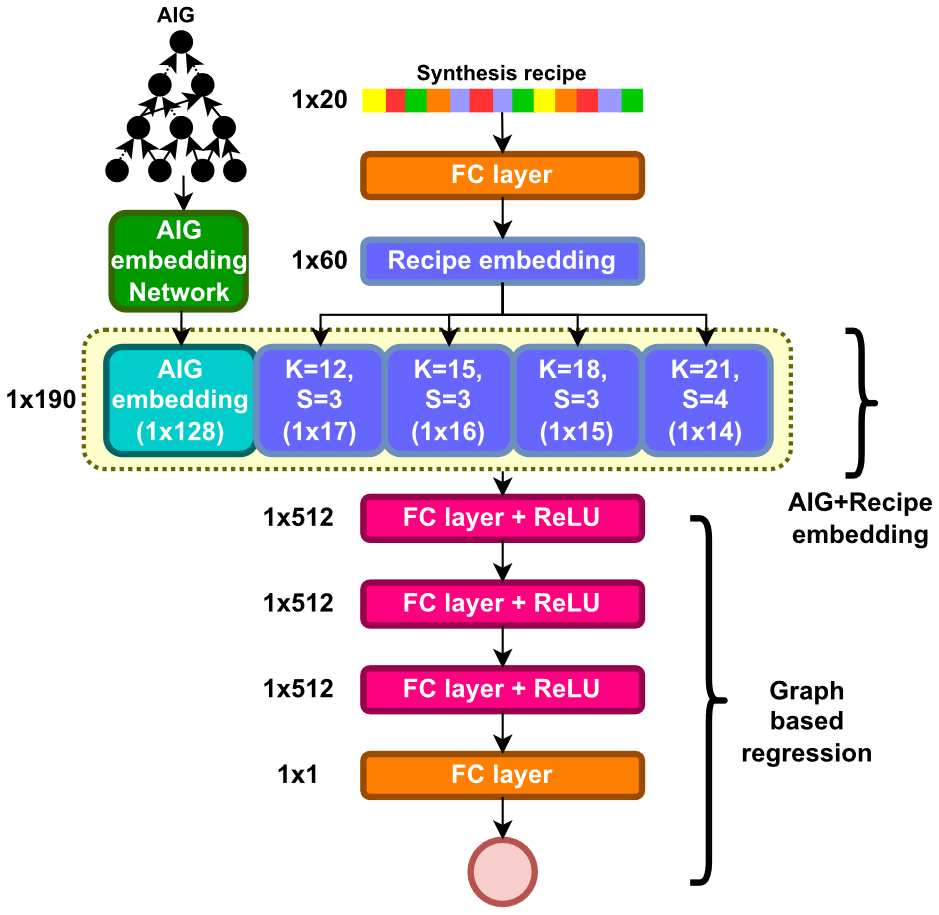
\includegraphics[width=0.7\linewidth]{./figs/LS-Bulls-Eye-QoR_predictor.png}
    \caption{基于AIG和GCN的序列质量预测器}
    \label{LS:Bulls-Eye:Fig:QoR_predictor}
\end{figure}

\begin{figure}[!htbp]
    \centering
    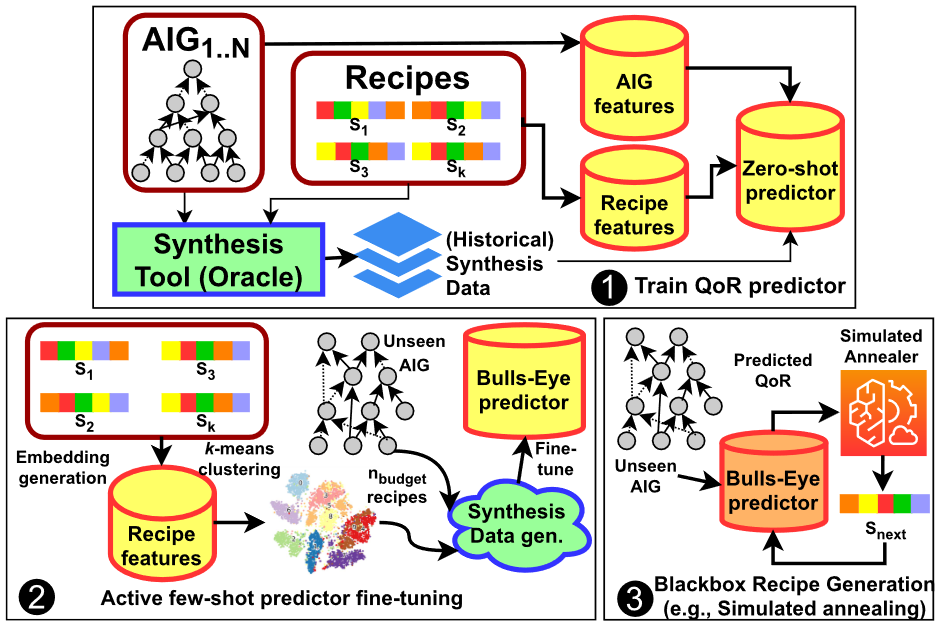
\includegraphics[width=0.9\linewidth]{./figs/LS-Bulls-Eye-overall_framework.png}
    \caption{Bulls-Eye整体框架图}
    \label{LS:Bulls-Eye:Fig:overall_framework}
\end{figure}

文献\cite{LS:Bulls-Eye}首先利用GCN基于AIG提出了一个序列质量预测器,总体结构如图\ref{LS:Bulls-Eye:Fig:QoR_predictor}所示。预测器的输入包括AIG和优化命令序列(图中的Synthesis recipe),两者分别通过AIG嵌入网络和序列嵌入网络进行嵌入,拼接后经过四层全连接层进行输出。之后,在基于小型电路集上对预测器进行训练后,面对新的大型电路,通过主动学习(Active learning)的方式对预测器进行微调,以提高对新电路的预测准确率。最后,基于微调后的预测器,利用模拟退火算法对新电路生成一个高质量的优化序列,整体框架命名为Bulls-Eye,流程如图\ref{LS:Bulls-Eye:Fig:overall_framework}所示。Bulls-Eye的预测器在基于44个开源电路设计组成的数据集上进行训练,实验表明,训练后的模型在新的大型电路的序列质量预测任务中表现良好,微调后的模型准确率进一步上升。

\subsubsection{多种DAG联合优化}

基于MIG对算术电路的综合及映射效果比AIG更好这一特点,文献\cite{LS:LSOracle}提出了LSOracle,是第一个同时采用多种DAG形式对布尔逻辑电路进行表示和优化的开源异构逻辑综合框架。

\begin{figure}[!htbp]
    \centering
    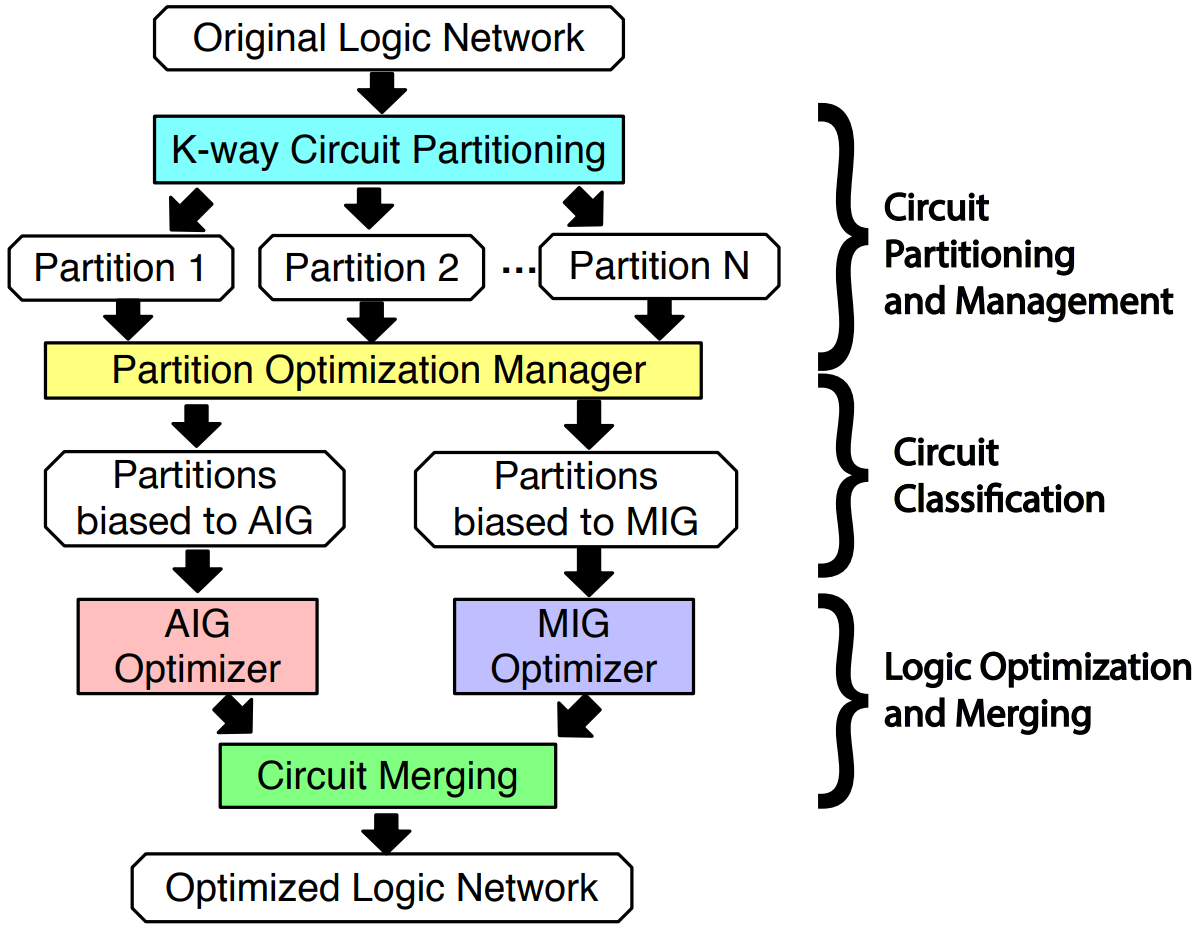
\includegraphics[width=0.7\linewidth]{./figs/LS-LSOracle-flow.png}
    \caption{LSOracle流程图}
    \label{LS:LSOracle:Fig:flow}
\end{figure}

图\ref{LS:LSOracle:Fig:flow}展示了LSOracle的工作流程图,输入电路首先被转换成AIG,然后变成超图。
接着利用开源的超图划分工具KaHyPar\cite{KaHyPar}将其分割成多个子图,子图之前存在松散的连接。
之后,分类引擎会利用二维图片对子图进行表示,并利用神经网络对图片进行分类,对每个子图挑选出一种最适合的DAG表示(AIG或MIG)并优化。具体来讲,设$B=\{0,\ 1\}$,一个$n$输入的布尔函数是一个从$B^n$到$B$的映射:$f: B^n \rightarrow B$。因此,一个$n$输入的布尔函数可以由一个$n$维空间表示,卡诺图是一种利用二维空间完成$n$维空间映射的表示形式。受卡诺图启发,LSOracle提出了一种用二维图片来表示逻辑函数的方法,命名为KMImage(Karnaugh-Map Image)。
\begin{figure}[!htbp]
    \centering
    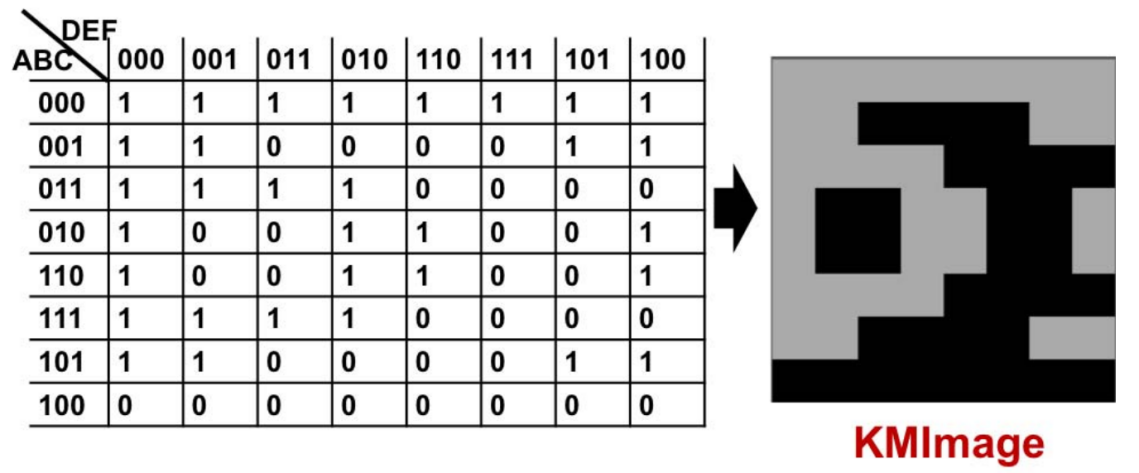
\includegraphics[width=0.9\linewidth]{./figs/LS-LSOracle-KMImage.png}
    \caption{将卡诺图转变为KMImage的示例}
    \label{LS:LSOracle:Fig:KMImage}
\end{figure}
图\ref{LS:LSOracle:Fig:KMImage}展示了一个将卡诺图转换为KMImage的例子,在KMImage中,每个像素点对应卡诺图中的一个输出,卡诺图中数值为1的输出在KMImage中以灰色像素表示,卡诺图中数值为0的输出在KMImage中以黑色像素表示。这种表示方法类似于MNIST\cite{DNN:LeNet_MNIST}数据集中的图片表示方法。在MNIST中,每张图片包含28×28个像素点,由黑白两种颜色组成。
通过将布尔函数转换为二维图片,能够利用计算机视觉领域成熟的研究方法对KMImage的特征进行识别和分类,挑选出最适合对应真值表实现的DAG格式。
一个$N \times N$大小的KMImage可以表示任意一个输入数为$2log_2 N$的逻辑函数,易知同一逻辑函数在改变输入顺序后对应不同的KMImage(除非函数是对称的),有可能导致分类结果不一致。然而,一个逻辑函数只会对应一种最优的DAG实现,分类错误会导致电路性能的下降,LSOracle并没有考虑改变输入顺序后有可能得到更优DAG分类的情况,这是其考虑不周的地方。

超图划分后的子图往往是多输出函数,KMImage只能表示单输出函数,为了解决多输出函数子图的分类问题,LSOracle采用了一种计分机制。具体来讲,分类引擎根据所有主要输出节点的最大逻辑锥(见\ref{MFFC}有关锥的定义)得到多个KMImage并赋予不同的权重,节点数目越多、网络深度越大的锥的权重越大。在对每个KMImage进行分类之后,分别计算不同DAG的总得分,得分最高的DAG作为该子图的最终分类结果,计算公式如下所示:
\begin{equation}
\label{LS:LSOracle:Eq:score}
score = \sum_{i=1}^{m} ( W_{ni} * N_i +W_{di} *D_i )
\end{equation}
式中$m$是子图的主要输出数,也是KMImage的个数;$N_i$和$W_{ni}$分别是第$i$个KMImage对应的锥的节点数和节点数权重;$D_i$和$W_{di}$分别是第$i$个KMImage对应的锥的深度和深度权重。LSOracle的分类器采用大小为$256 \times 256$的固定尺寸的KMImage,可以表示不超过16个输入的逻辑函数。对于小于16个输入的逻辑函数,通过随机填充的方法将KMImage扩展到$256 \times 256$大小。对于超过16个输入的逻辑函数,直接通过启发式算法对其进行分类:如果一个锥的逻辑深度超过所在子图逻辑深度的40\%,那么该锥被分类到MIG,否则被分类到AIG,所有锥分类完成后根据式\eqref{LS:LSOracle:Eq:score}计算不同DAG的得分,最终得到该子图的分类结果。一旦一个子图分类完成,该子图立刻被转化成对应的DAG格式,由预先指定的优化脚本进行优化,当所有的子图优化完成后,合并优化后的子图并将整个电路转换成MIG,进行最后的优化并输出。

LSOracle的分类算法具有一定的局限性:(1)KMImage具有固定尺寸,只能表示不大于16个输入数的逻辑函数,对小于16个输入数的布尔函数采用“随机补全”的办法,存在不确定性,影响分类精度;(2)划分后的子图往往是多输出的,然而KMImage只能表示单输出函数,即使能够利用多个KMImage对子图进行表征,但多个KMImage对应的布尔网络(锥)之间存在重复的节点,带来了重复的计算,影响分类精度。解决这两个问题可以采用基于图神经网络(Graph Neural Network, GNN)对子图进行分类的方法,GNN不受电路规模和输出个数的影响,能够极大地提高分类效率。

\subsection{研究动机}

目前已有的序列优化方法\cite{LS:BOiLS,LS:DRiLLS}在针对大规模电路进行探索时迭代速度慢,无法在有限地时间内得到高质量的输出结果,尽管有工作\cite{LS:Bulls-Eye}在基于图神经网络训练一个预测器后利用主动学习的方法能够在较短时间内应用到大网络上,但预测质量往往不如直接探索的方法,同时预测器的搜索空间是预先固定的,无法进行灵活调整。另外,已有的方法都是直接将一个优化序列应用于整个网络,考虑到电路的算术逻辑部分和控制逻辑部分有不同的特性\cite{LS:MIG},网络的不同部分可能适用于不同的序列。

文献\cite{LS:LSOracle}利用超图划分的方法对布尔网络进行分割,并对划分后的子网络选择合适的DAG进行优化,但由于划分后每个子网络的输入信号的到达时间可能不为0,这导致对子网络进行优化时的关键路径可能并不是真实的关键路径,同时超图划分的目标只是最小化割边权重和或子图连通性,并没有考虑节点处于不同子图会带来不同优化效果的影响,且不同DAG的优化引擎质量不一致,这些原因加起来导致合并后的网表经过评估后优势不大。因此需要针对大规模网络提出一个基于高质量划分的序列探索方法,既能充分利用现代CPU架构的多核特性提高探索效率,又能保证合并后优化质量的提升。

\subsection{研究内容与创新点}

\begin{figure}[!htbp]
    \centering
    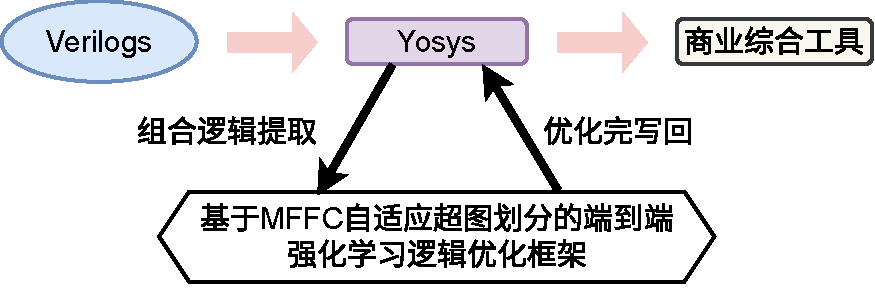
\includegraphics[width=\linewidth]{./figs/LS-MFFC_rl.pdf}
    \caption{本文提出的逻辑优化框架流程图}
    \label{LS:MFFC_rl}
\end{figure}

本文提出并开源了一个基于MFFC自适应超图划分的端到端强化学习逻辑优化框架,该框架基于Yosys\cite{LS:yosys}和ABC\cite{LS:ABC}实现。首先利用Yosys对电路进行读入和解析,接着将电路中的组合逻辑提取出来。基于文献\cite{Moucheng_Yang}的发现,利用ABC将提取的组合逻辑转换成AIG并“自然划分”,得到一个或多个AIG簇(若AIG簇只有一个,则该AIG簇为原AIG),簇与簇之间互相没有任何连接。对“自然划分”后规模仍然较大的簇,利用MFFC遍历将簇转换成以MFFC为节点的超图。之后利用开源的超图划分工具KaHyPar\cite{KaHyPar}采用多层划分的方法对MFFC超图进行划分,即得到AIG簇的划分。划分完成后,对所有的子电路并行地利用提出的强化学习序列优化方法在给定的时间内进行搜索。最后合并所有基于找到的高质量序列进行优化后的子电路,写回到Yosys,和时序逻辑一起输出,由商业综合工具进行评估,整体流程如图\ref{LS:MFFC_rl}所示。主要创新点如下:
\begin{itemize}
    \item 提出了一个开源的应用于大型电路的端到端强化学习逻辑优化框架,该框架在对布尔网络进行分割后并行地利用强化学习方法进行序列探索,充分利用现代CPU的多核特性,提高探索效率;
    \item 与不分割相比,划分后能够对大网络的不同区域进行充分探索,避免了基于整个网络进行优化带来的局限性;
    \item 基于超过150个电路的商业综合工具的评估结果显示,与ABC resyn2相比,面积延迟积平均提高了5.17\%。
\end{itemize}

\subsection{研究方法}

(1)自然划分

本文首先利用Yosys对Verilog进行解析,将电路中的组合逻辑和时序逻辑分开,其中,寄存器的输入会变成组合逻辑的输出,寄存器的输出会变成组合逻辑的输入。之后基于文献\cite{Moucheng_Yang}的发现,将提取出的组合逻辑通过ABC读入,转成AIG,并识别出AIG中所有互相之间没有连接的逻辑簇,按照簇将AIG进行分割,易知切割的边数为0,且分割得到的所有簇的主要输入要么来源于电路的输入、要么来源于寄存器的输出,因此所有簇的输入延迟均为0。

(2)基于MFFC的超图划分

自然划分后,有可能会存在过大的簇,对于过大的簇,首先对所有的节点遍历并计算MFFC,根据\ref{MFFC}的内容可知两个MFFC要么不相交、要么一个包含另一个,当两个MFFC存在包含关系时,保留大的MFFC作为超图中的节点。同时,一个MFFC内节点的值只会影响到该MFFC的根节点和根节点的传递扇出,因此与直接对簇进行划分相比,MFFC超图的出现相当于在划分前将一些应该一起优化的AIG节点捆绑在一起,减少文献\cite{LS:LSOracle}中直接对AIG进行划分带来的缺点。
MFFC超图形成后,对其采用开源的超图划分工具\cite{KaHyPar}进行分割,为了保证分割后每个子图的AIG规模大致相等,MFFC超图中每个节点都有一个权重值,大小为该MFFC的节点数。

(3)提出的强化学习方法

DRiLLS\cite{LS:DRiLLS}在序列探索过程中每次运行一个优化命令都需要保存一个中间文件,效率较低。本文提出并开源了一个新的强化学习逻辑综合方法,该方法基于OpenAI Gym\cite{AI:gym}和Stable Baselines3\cite{AI:stable-baselines3}实现,支持ABC\cite{LS:ABC}、Cirkit\cite{LS:cirkit}、iMAP\cite{LS:iMAP}三个学术界主流的逻辑综合工具,能够完成以逻辑优化、LUT映射、ASIC映射为目标的序列探索任务。

\subsection{实验结果}

对来自OPDB\cite{LS:OPDB}、VTR\cite{FPGA:vtr8}、Koios\cite{FPGA:Koios}、EPFL\cite{LS:EPFL_benchs_iwls,LS:EPFL_benchs_github}、IWLS05\cite{LS:iwls05}、QUIP\cite{LS:quip}等超过150个不同规模的电路进行广泛测试,对提取的组合逻辑网表分别用ABC resyn2、BOiLS\cite{LS:BOiLS}、DRiLLS\cite{LS:DRiLLS}、LSOracle\cite{LS:LSOracle}、以及本文提出的方法在Intel Xeon处理器上利用200个CPU核进行优化,其中BOiLS和DRiLLS使用单线程运行,运行时间由下式确定:
\begin{equation}
    runtime = \lceil \frac{N_{p}}{200} \rceil * 2 h
\end{equation}
其中$N_{p}$代表根据本文提出的方法进行“自然划分”和MFFC超图划分后所有的子电路的总数,$\lceil \ \rceil$表示向上取整。
优化完成后和时序逻辑合并输出,利用Synopsys Design Compiler (DC) S-2021.06-SP5在一个开源的7nm工艺库\cite{ASAP7_github}进行综合,获得面积延迟积(Area Delay Product, ADP)进行比较。为了避免DC的优化对结果带来影响,将电路的时钟频率约束设为0,同时最小化面积(set\_max\_area 0),并使用“compile”命令进行映射。
注意本文并没有考虑划分消耗的时间,对于一个拥有百万个AIG节点的组合逻辑网络来说,“自然划分”和MFFC超图划分所花费的时间总共在10h左右。

\begin{table*}[!htb]
    % \renewcommand{\arraystretch}{1.4}
    % \setlength\tabcolsep{3.76pt}
    \caption{基于不同方法得到的面积、延迟和ADP的平均百分比提升}
    \begin{center}
    \scalebox{0.9}{
        \begin{tabular}{|c|c|c|c|c|c|}
        \hline
        最大的$n$个电路 &  & LSOracle\cite{LS:LSOracle} & BOiLS\cite{LS:BOiLS} & DRiLLS\cite{LS:DRiLLS} & 本文的方法 \\
        \hline
        \multirow{3}{*}{10} & Area(\%) & 1.57 & -10.69 & \textcolor{red}{-12.00} & -11.13 \\
        \cline{2-6}
        & Delay(\%) & 12.10 & 0.69 & \textcolor{red}{-2.52} & -0.23 \\
        \cline{2-6}
        & ADP(\%) & 14.35 & -10.45 & \textcolor{red}{-14.11} & -11.52 \\
        \hline
        \multirow{3}{*}{20} & Area(\%) & 1.29 & -5.80 & \textcolor{red}{-6.58} & -6.55 \\
        \cline{2-6}
        & Delay(\%) & 13.61 & -0.69 & -1.74 & \textcolor{red}{-1.78} \\
        \cline{2-6}
        & ADP(\%) & 15.67 & -6.72 & -8.11 & \textcolor{red}{-8.37} \\
        \hline
        \multirow{3}{*}{30} & Area(\%) & 5.03 & -5.78 & \textcolor{red}{-6.19} & -4.87 \\
        \cline{2-6}
        & Delay(\%) & 11.12 & -0.08 & 0.09 & \textcolor{red}{-0.82} \\
        \cline{2-6}
        & ADP(\%) & 17.55 & \textcolor{red}{-5.95} & -5.88 & -5.73 \\
        \hline
        \multirow{3}{*}{40} & Area(\%) & 4.10 & -5.04 & -5.47 & \textcolor{red}{-5.50} \\
        \cline{2-6}
        & Delay(\%) & 8.90 & -0.55 & -0.29 & \textcolor{red}{-1.49} \\
        \cline{2-6}
        & ADP(\%) & 14.08 & -5.41 & -5.46 & \textcolor{red}{-6.75} \\
        \hline
        \multirow{3}{*}{所有($\ge 150$)} & Area(\%) & 2.08 & -3.29 & -3.61 & \textcolor{red}{-3.85} \\
        \cline{2-6}
        & Delay(\%) & 3.81 & -0.64 & -0.30 & \textcolor{red}{-1.70} \\
        \cline{2-6}
        & ADP(\%) & 6.16 & -3.68 & -3.73 & \textcolor{red}{-5.17} \\
        \hline
        \end{tabular}
    }
        \label{LS:MFFC_rl:Table:results}
        \end{center}
\end{table*}

表\ref{LS:MFFC_rl:Table:results}展示了以ABC resyn2为标准进行归一化的平均百分比提升,正数表示变差,负数表示改进,标红的数字代表每一行对应的指标中不同方法得到的最好结果。
可以看到,LSOracle\cite{LS:LSOracle}的效果最差,数据显示,与ABC resyn2相比,LSOracle在最大的10、20、30、40个电路上面积和延迟的平均百分比没有任何提升,反而在变差,这可能是因为尽管LSOracle使用了多种DAG对电路进行表示,但不同DAG的优化引擎效果不一致,导致网表合并后并没有明显的改进,同时不同DAG的节点实现成本不一样,比如AIG中每个节点代表一个2输入与门,而MIG中每个节点代表一个3输入的Majority门,这导致MIG中节点的实现成本更高,无法简单通过比较同一电路在不同DAG实现下的节点数和级数来判断DAG映射后的好坏。与ABC resyn2相比,超过150个电路的测试结果显示,LSOralce的面积、延迟、ADP分别变差了2.08\%、3.81\%、6.16\%,且电路越大LSOracle的效果越差,比如LSOracle的ADP比ABC resyn2在最大的10个电路上平均退步了14.35\%。
BOiLS和DRiLLS的结果是在没有划分的情况下直接对整个组合逻辑网表进行优化得到的,可以看到DRiLLS对大规模电路的探索效果更好,与BOiLS相比,DRiLLS在最大的10个电路上的面积、延迟、ADP分别平均提升了1.31\%、3.21\%、3.66\%,且在最大的20个电路的表现也优于BOiLS。
本文提出的基于MFFC自适应超图划分的端到端强化学习逻辑优化方法在大电路上的表现不弱于BOiLS,最大的10个电路的面积、延迟、ADP相比BOiLS分别平均提升了0.44\%、0.92\%、1.07\%。
基于全部的超过150个电路的实验结果显示,本文提出的方法效果最好,与ABC resyn2、BOiLS、DRiLLS相比ADP分别提升了5.17\%、1.49\%、1.44\%。

考虑到数据是基于大量的用例通过商业综合工具评估得到的,因此实验结果能够代表真实的应用场景,每个电路具体的面积和延迟数据见附录\ref{所有电路在不同优化方法下的面积和延迟}。


\section{基于近似乘法器库面向DNN加速器的近似逻辑综合}

\subsection{研究背景}

即使设计的近似乘法器在经过评估后硬件开销较低,但基于该乘法器设计的DNN加速器可能硬件成本并不领先。例如,在图\ref{AC:AM:Adapt:Fig:LeNet_PDA_accuracy}中,PPAM(1,1)的PDA比XFYW和XWYF都要高,但在如图\ref{AC:AM:Adapt:Fig:Acc_TASU}所示的基于不同乘法器的TASU加速器的\cite{Accelerator:JiaoLi}硬件开销比较中,基于PPAM(1,1)的设计比基于乘法器\emph{`A'}、\emph{`B'}、\emph{`C'}的PDA都要低,这是因为当近似乘法器作为一个模块放在电路中时,EDA工具能够根据不同的电路执行不同的优化,因此有必要对基于不同近似乘法器的DNN加速器的硬件成本进行探究。

\subsection{研究内容}

\subsubsection{研究方法}

将提出的基于MFFC自适应超图划分的端到端强化学习逻辑优化框架与近似乘法器库结合,针对DNN硬件加速器,本文首先对图\ref{AC:AM:Adapt:Fig:LeNet_PDA_accuracy}中共68个XWYF近似乘法器利用DC在7nm工艺库\cite{ASAP7_github}上基于2GHz的时钟频率约束进行综合以获取PDA,找到位于帕累拖前沿的乘法器;之后对基于不同乘法器的68个卷积操作加速单元SC\cite{Accelerator:SC}利用提出的开源逻辑优化框架进行优化,获取ADP并比较结果。


\subsubsection{实验结果}

\begin{figure}[!htb]
    \centering
    \subfigure[XWYF乘法器的评估结果]{
    \label{AC:ALS:Fig:LeNet_XWYF}
    \begin{minipage}[t]{0.48\linewidth}
    \centering
    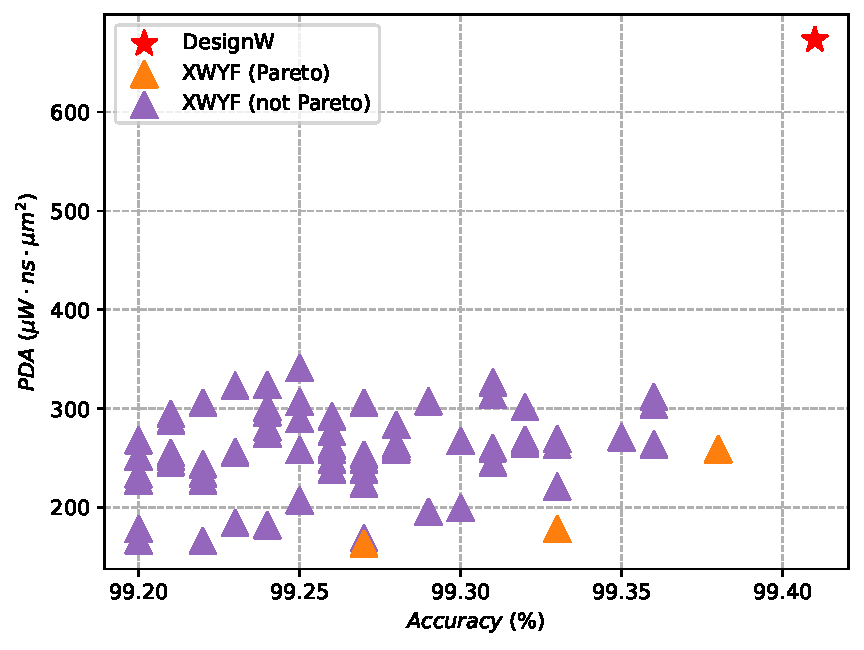
\includegraphics[width=\linewidth]{figs/LeNet_XWYF_PDA.pdf}
    \end{minipage}
    }
    \subfigure[基于XWYF实现的卷积加速器的评估结果]{
    \label{AC:ALS:Fig:SC}
    \begin{minipage}[t]{0.48\linewidth}
    \centering
    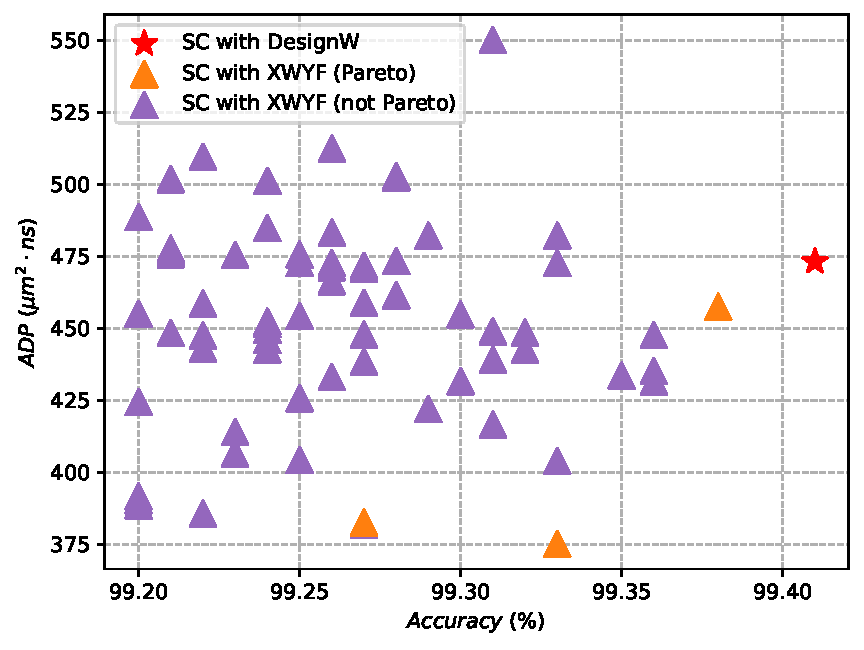
\includegraphics[width=\linewidth]{figs/SC_LeNet_XWYF_ADP.pdf}
    \end{minipage}
    }
\caption{XWYF乘法器的评估结果以及基于XWYF实现的卷积加速器的评估结果}
\label{AC:ALS:Fig:SC_LeNet_XWYF}
\end{figure}

图\ref{AC:ALS:Fig:SC_LeNet_XWYF}展示了68个XWYF乘法器的评估结果以及基于XWYF实现的68个卷积加速器SC\cite{Accelerator:SC}的评估结果,作为对比,基于DesignWare库\cite{IP:DesignWare}实现的精确乘法器DesignW也被纳入比较。图\ref{AC:ALS:Fig:LeNet_XWYF}中共有3个乘法器位于帕累拖前沿,以黄色三角形表示,对应的SC实现在图\ref{AC:ALS:Fig:SC}中也以黄色三角形表示。一个有意思的现象是,虽然DesignW的单独评估结果显示其PDA较高,但基于DesignW实现的SC模块的硬件开销却优于相当一部分的XWYF乘法器,这说明了近似乘法器库在使用时不能简单地根据单独的硬件成本直接选择,而是应该进行多次尝试后决定。
图\ref{AC:ALS:Fig:SC}表明,基于3个帕累拖最优的乘法器的SC实现仍然位于帕累拖前沿,因此当给定一个近似乘法器库进行综合时,可对库中位于帕累拖前沿的乘法器进行一定次数的随机搜索,综合比较后选择最好的那个进行实现。

\section{本章小结}

本章首先介绍了基于MFFC自适应超图划分的端到端强化学习逻辑优化框架,该框架基于Yosys和ABC实现,首先利用Yosys对电路进行读入和解析,接着将电路中的组合逻辑提取出来并划分,划分完成后采用强化学习方法对所有的子电路并行地进行序列寻优,最后通过商业综合工具进行评估。基于超过150个电路的实验结果显示,与ABC的脚本resyn2相比,面积延迟积平均提高了5.17\%。之后将框架与近似乘法器库结合,对基于不同近似乘法器的DNN硬件加速器进行研究,结果显示乘法器和加速器之间的性能收益存在不匹配的现象,即乘法器本身的硬件开销低,基于该乘法器实现的加速器的硬件开销不一定低,因此近似乘法器库在使用时不能简单地根据乘法器的单独硬件成本直接选择,而是应该进行多次尝试后决定。